% ===============================
%          Chapter 2A.2
%  Cell Transport and Diffusion
%     Created by Michael Tang
%           2025.02.16
% ===============================

\subsubsection{2A.2 Cell Transport and Diffusion}
\paragraph{Types of membrane transport}
Substance move across membranes via passive transport (no energy required / no ATP used) or active transport (energy required /
ATP used).
\begin{itemize}
    \item \textbf{Diffusion:} No energy required / no ATP used. Molecules move from high concentration to low concentration.
    Random movement of molecules.
    \item \textbf{Facilitated diffusion:} No energy required / no ATP used. Molecules move from high concentration to low
    concentration. Uses carrier or \underline{channel proteins} (管道蛋白).
    \item \textbf{Osmosis:} No energy required / no ATP used. Movement of water molecules from high concentration to low
    concentration. Water moves through a selectively \underline{permeable membrane} (渗透膜).
    \item \textbf{Active transport:} Energy required / ATP used. Molecules move from low concentration to high concentration.
    Uses carrier proteins.
    \item \textbf{\underline{Endocytosis} (内吞作用):} Energy required / ATP used. Molecules move into the cell.
    \underline{Vesicle} (囊泡) forms around the substance.
    \item \textbf{\underline{Exocytosis} (胞吐作用):} Energy required / ATP used. Molecules move out of the cell.
    Vesicle fuses with the cell membrane.
\end{itemize}

\paragraph{Passive Diffusion}
No ATP required - molecules move down a concentration gradient.
\begin{itemize}
    \item \textbf{Diffusion}
    \begin{itemize}
        \item Movement of molecules from high concentration to low concentration due to \underline{kinetic energy} (动能).
        \item Example: Oxygen (\ce{O2}) and carbon dioxide (\ce{CO2}) diffuse freely across the cell membrane.
    \end{itemize}
    \begin{figure}[H]
        \centering
        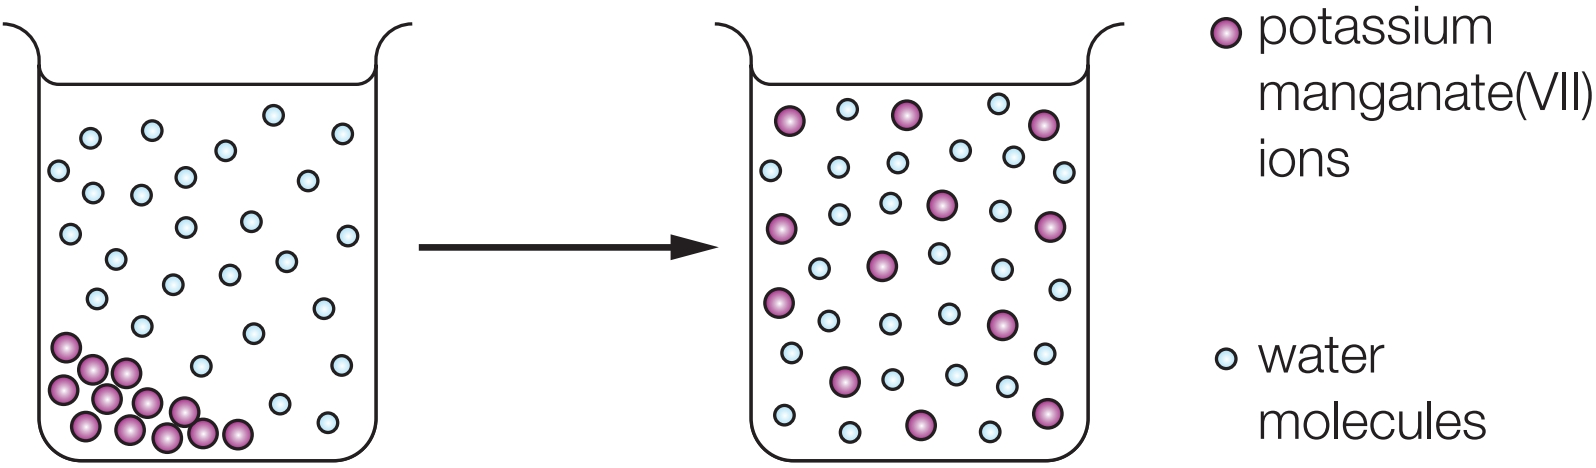
\includegraphics[scale=0.12]{Biology/2A/Images/2A-2-1.png}
        \caption{If the beaker is left to stand, diffusion takes place as the random movement of both the water and the
        \underline{potassium manganate (VII) ions} (\ce{MnO4^-}) ensures that they become evenly mixed.} 
    \end{figure}
    \item \textbf{Facilitate Diffusion}
    \begin{itemize}
        \item \textbf{Larger / polar molecules} (e.g., glucose, amino acids) need carrier or channel proteins.
        \item \textbf{Channel proteins}
        \begin{itemize}
            \item Specific to certain ions / molecules.
            \item Can be gated (open / close in response to signals).
        \end{itemize}
        \textbf{Carrier proteins:} Bind to a molecule and change shape to move it across the membrane.
    \end{itemize}
    \begin{figure}[H]
        \centering
        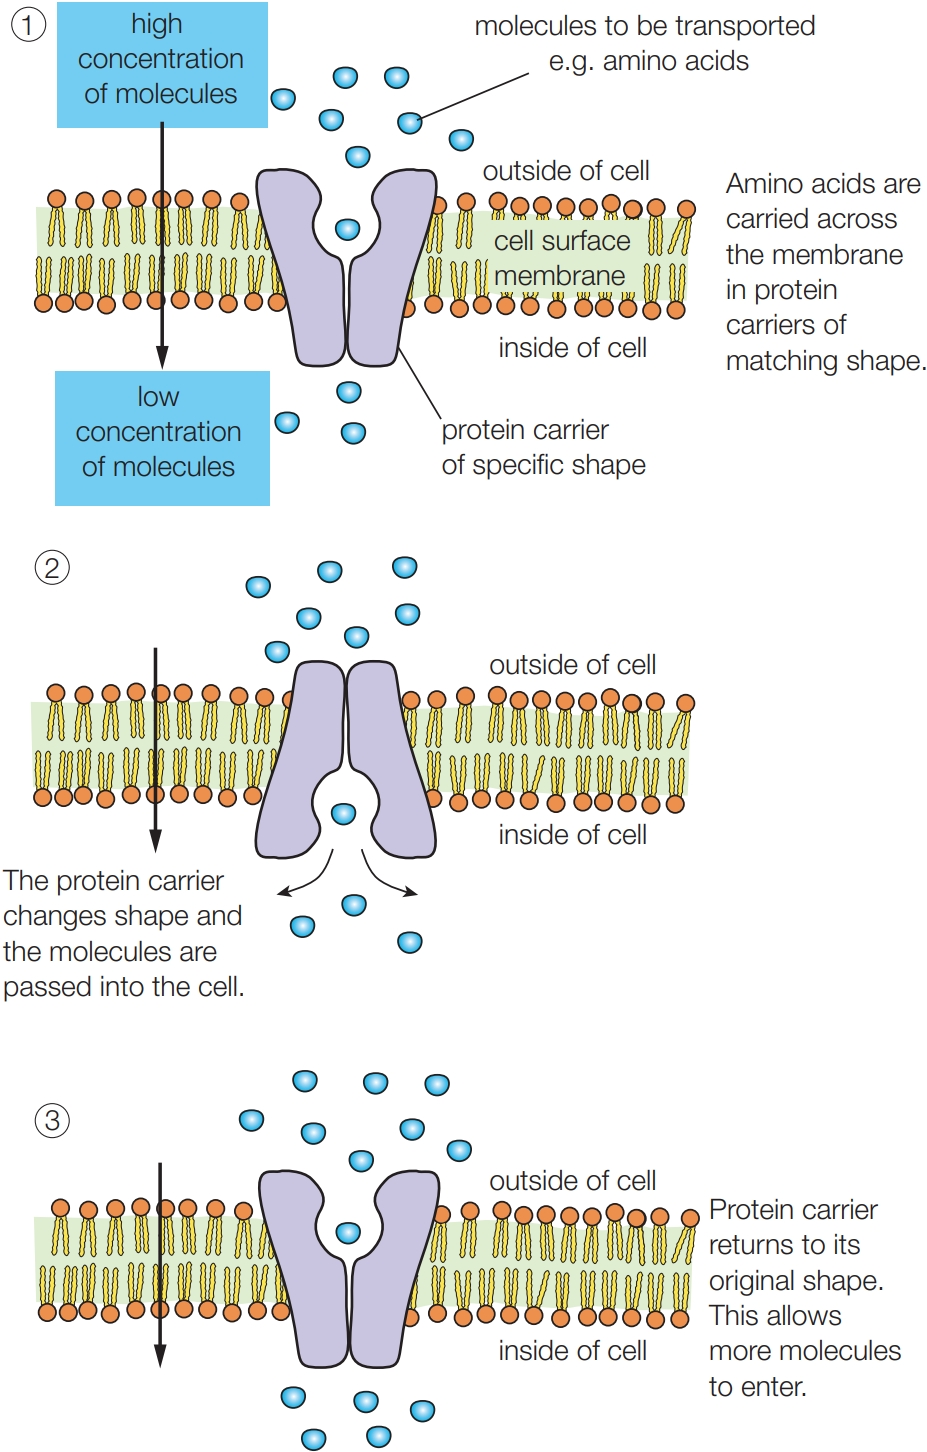
\includegraphics[scale=0.25]{Biology/2A/Images/2A-2-2.png}
        \caption{Facilitated diffusion acts as a ferry across the lipid membrane sea. It is not an active process, so it can only
        work when the concentration gradient is in the right direction.} 
    \end{figure}
    \item \textbf{Osmosis}
    \begin{itemize}
        \item The movement of water molecules from a high water potential to a low water potential.
        \item Occurs through a partially permeable membrane.
    \end{itemize}
\end{itemize}
\begin{figure}[H]
    \centering
    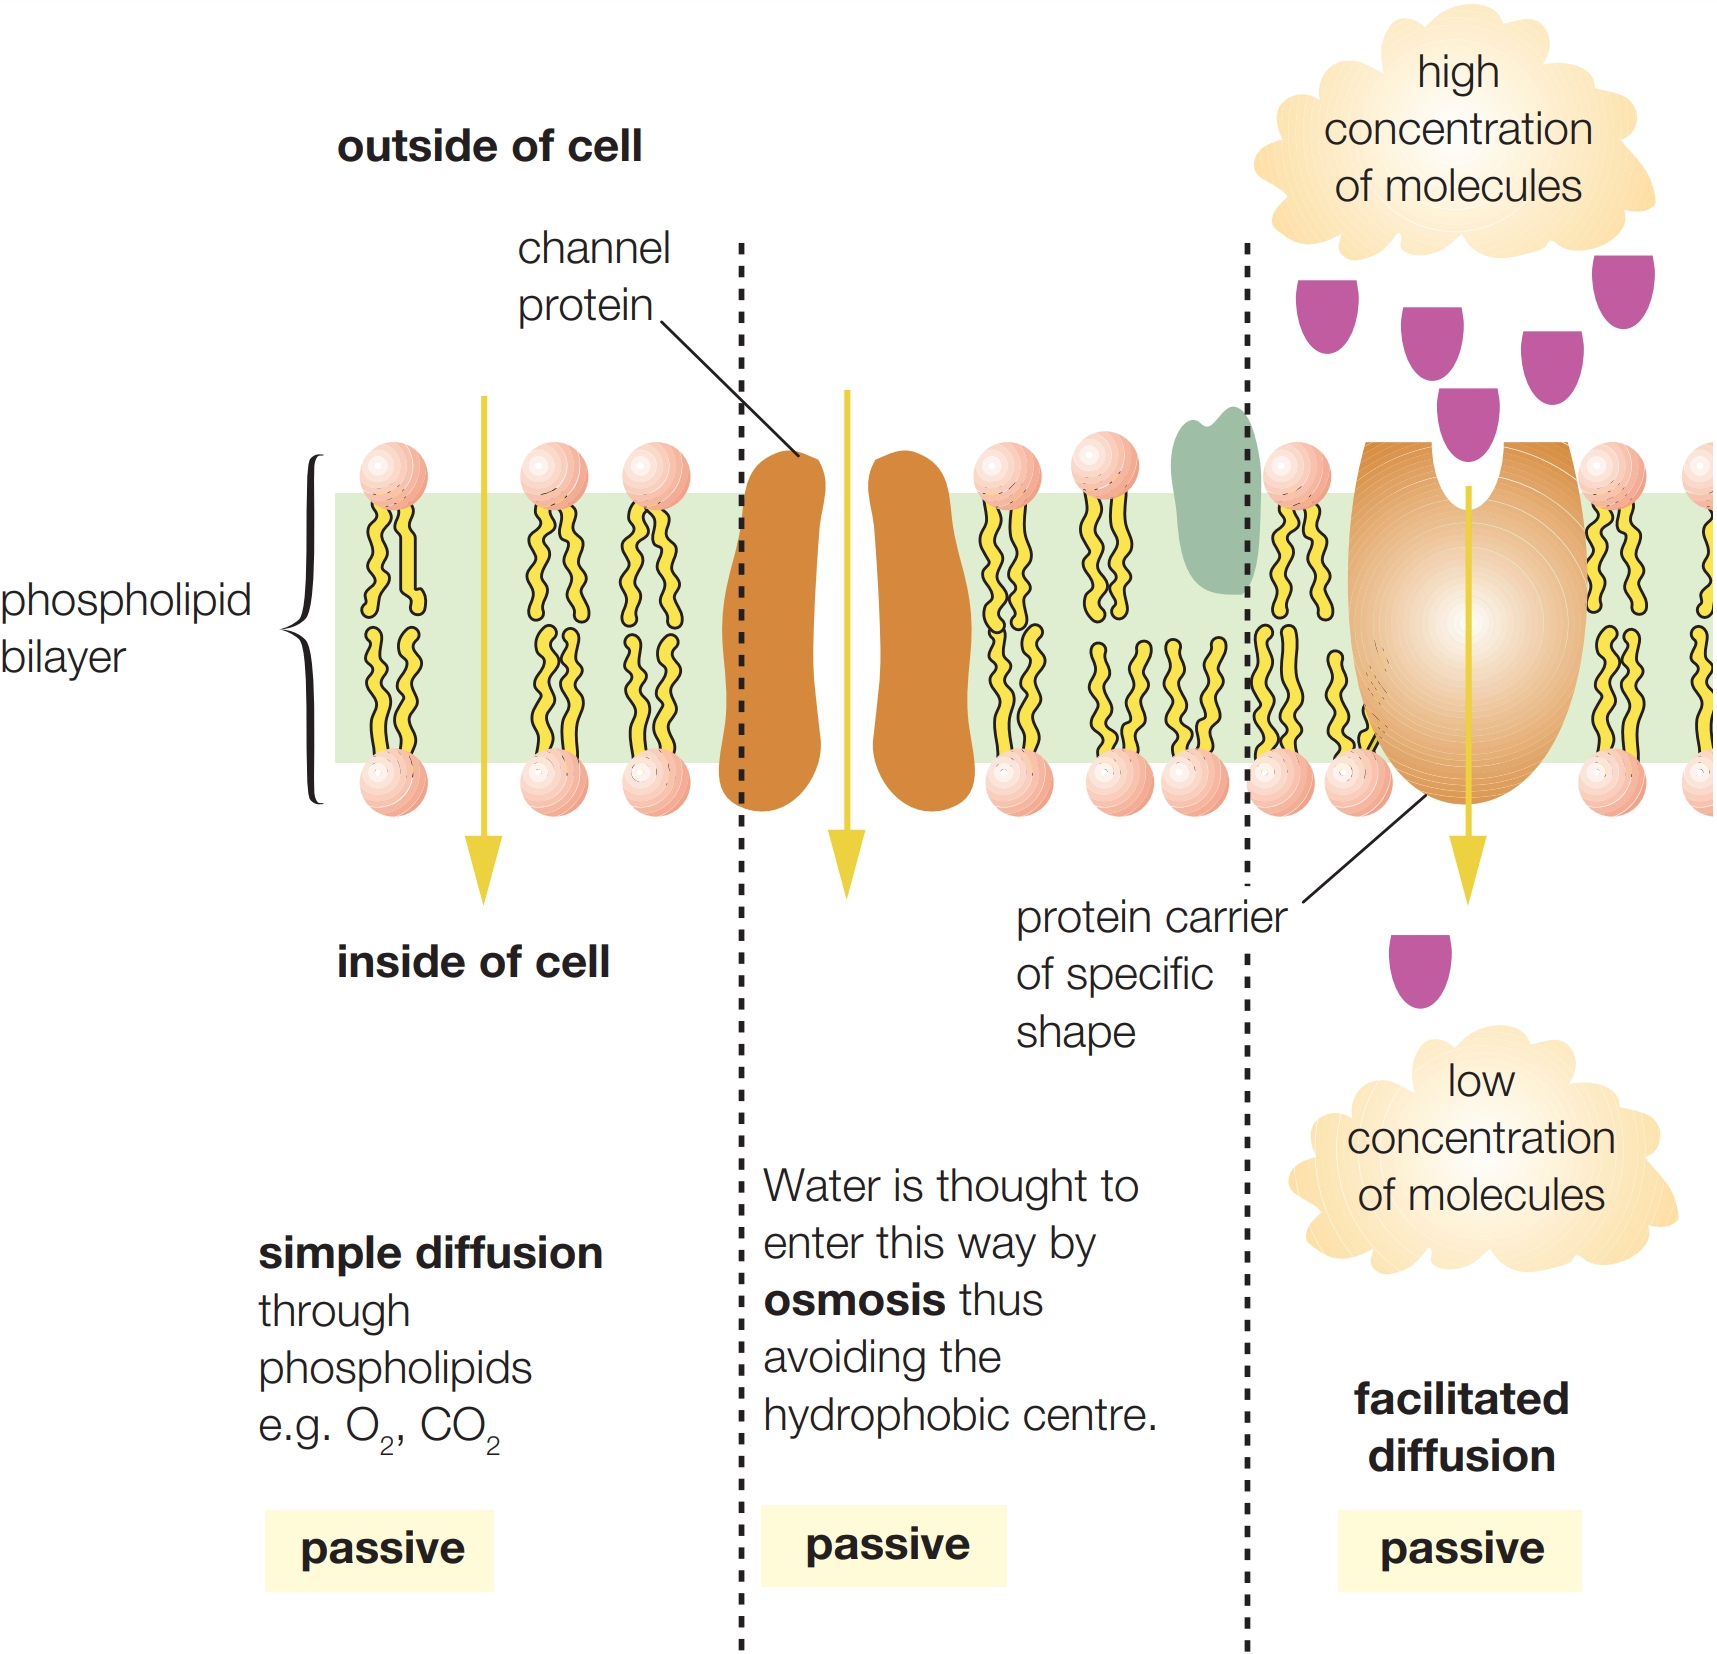
\includegraphics[scale=0.125]{Biology/2A/Images/2A-2-3.png}
    \caption{The main passive transport routes through a cell surface membrane.} 
\end{figure}

\paragraph{Active Transport (ATP Required)}
\begin{itemize}
    \item Moves molecules against the concentration gradient.
    \begin{itemize}
        \item Uses carrier proteins powered by ATP.
        \item Example: \underline{Sodium-potassium pump} \footnote{The sodium-potassium pump (\ce{Na^+} / \ce{K^+} pump) is a
        type of active transport that moves sodium (\ce{Na^+}) out of the cell and potassium (\ce{K^+}) into the cell, against
        their concentration gradients. This process requires ATP and helps maintain the resting membrane potential in nerve and
        muscle cells. The pump exchanges 3\ce{Na^+} ions out for 2\ce{K^+} ions in, making the inside of the cell more negative
        compared to the outside. This is essential for nerve impulse transmission, muscle contraction, and overall cell function.}
        (钾钠泵) in nerve cells.
    \end{itemize}
    \item \textbf{\underline{Endocytosis} (内吞作用) and \underline{Exocytosis} (胞吐作用)}
    \begin{itemize}
        \item \textbf{Endocytosis:} Large molecules enter the cell by forming vesicles.
        \item \textbf{Exocytosis:} Large molecules exit the cell by \underline{vesicle fusion} \footnote{Vesicle fusion is the
        process by which a vesicle, a small \underline{membrane-bound sac} (膜结合囊 / 膜包囊) containing substances, fuses with
        the cell membrane to release its contents into or out of the cell. This is a key mechanism in exocytosis (moving
        substances out of the cell) and endocytosis (bringing substances into the cell). During fusion, the vesicle membrane
        merges with the cell membrane, allowing the vesicle's contents, such as hormones or waste products, to be transported
        across the membrane. This process often requires energy in the form of ATP.} (囊泡融合) with the membrane.
        \item Example: Secretion of enzymes, hormones, \underline{neurotransmitters} \footnote{Neurotransmitters are chemical
        messagers that transmit signals across a \underline{synapse} (突触, the gap between two nerve cells). They are released
        from the \underline{axon terminal} (轴突终末) of a neuron and bind to \underline{receptors} (受体 / 感受器) on the
        \underline{dendrites} (树突) of the next neuron triggering a response. Neurotransmitters play a key role in nerve signals
        transmission, influencing functions like mood, movement, and \underline{cognition} (认知). Examples include
        \underline{dopamine} (多巴胺, related to reward and movement), \underline{serotonin} (血清素 / 五羟色胺, influences mood
        and sleep), and \underline{acetylcholine} (乙酰胆碱, involved in muscle contraction). The proper balance of
        neurotransmitters is essential for normal brain function} (神经递质).
    \end{itemize}
\end{itemize}

\paragraph{Exam Keys}
\begin{itemize}
    \item Diffusion = kinetic energy only, no ATP.
    \item Facilitated diffusion uses proteins but still no ATP.
    \item Active transport uses ATP and carrier proteins to move substances against a gradient.
    \item Endocytosis and exocytosis uses vesicles for bulk transport.
\end{itemize}